\documentclass[12pt, a4]{article}
\usepackage[english]{babel}
\usepackage[utf8x]{inputenc}
\usepackage{fullpage}
\usepackage{listings}
\usepackage{graphicx}
\usepackage{color}

%Syntax highlighting
\definecolor{blue-violet}{rgb}{0.54, 0.17, 0.89}
\definecolor{ao}{rgb}{0.0, 0.5, 0.0}
\definecolor{amaranth}{rgb}{0.9, 0.17, 0.31}
\definecolor{ballblue}{rgb}{0.13, 0.67, 0.8}
\definecolor{onyx}{rgb}{0.06, 0.06, 0.06}


\lstset{
  breaklines=true,                 % automatic line breaking only at whitespace
  captionpos=b,                    % sets the caption-position to bottom
  breakatwhitespace=false,
  keepspaces=true,
  numbers=left,
  numbersep=5pt,
  showspaces=false,
  showstringspaces=false,
  showtabs=false,
  tabsize=4,  
  backgroundcolor=\color{white},   % choose the background color
  commentstyle=\color{ao},    % comment style
  keywordstyle=\color{amaranth},    % keyword style
  stringstyle=\color{blue-violet},    % string literal style
  numberstyle=\tiny\color{ballblue},	   % number style
  basicstyle=\ttfamily\footnotesize\color{onyx} % size of fonts used for the code
}

%Document Header
\title{\textbf{Department of CSE\\SSN College of Engineering}}
\author{\textbf{Vishakan Subramanian - 18 5001 196 - Semester VI}}
\date{7 March 2021}

\begin{document}
\maketitle
\hrule
\section*{\center{UCS 1602 - Compiler Design}}
\hrule
\bigskip

%Assignment Details
\subsection*{\center{\textbf{Exercise 5: Implementation of Desk Calculator Using Yacc Tool}}}
\subsection*{\flushleft{Aim:}}
\begin{flushleft}
Write a Lex program to recognize relevant tokens required for the \textbf{Yacc} parser to implement desk calculator. Write the Grammar for the expression involving the operators namely, \(+ , - , * , / \), \string^ , \( ( , )  \). Precedence and associativity has to be preserved. Yacc is available as a command in Linux. The grammar should have non terminals E, OP and a terminal id.
\\
Verify your calculator with the following inputs:
\begin{enumerate}
\item $3+9$
\item $3+9*6$
\item $(3+4)*7$
\item $(3-4)+(7*6)$
\item $5/7+2$
\item $(4^2)^1$
\item $(2^3)^2$
\end{enumerate}

\end{flushleft}

%Code
\newpage
\subsection*{\flushleft{Code - Yacc Parser File:}}
\begin{flushleft}
\lstinputlisting[language = C]{Calc.y}
\end{flushleft}

%Code
\newpage
\subsection*{\flushleft{Code - Lex Grammar File:}}
\begin{flushleft}
\lstinputlisting[language = C]{Calc.l}
\end{flushleft}

%Output
\newpage
\subsection*{\flushleft{Output 1:}}
\begin{figure}[h]
\centering
\caption{Console Output - 1.}
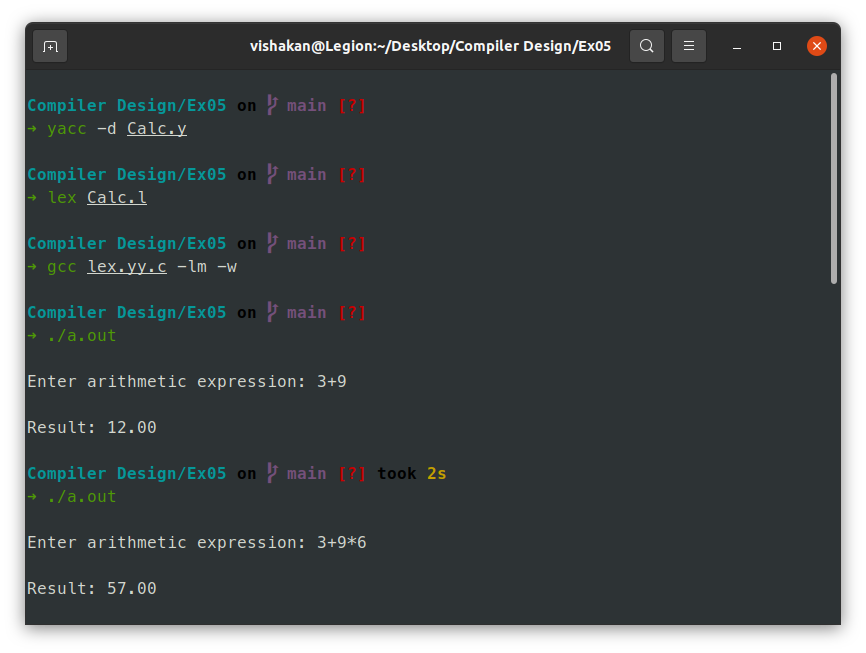
\includegraphics[scale= 0.5]{Output1.png}
\end{figure}

%Output
\newpage
\subsection*{\flushleft{Output 2:}}
\begin{figure}[h]
\centering
\caption{Console Output - 2.}
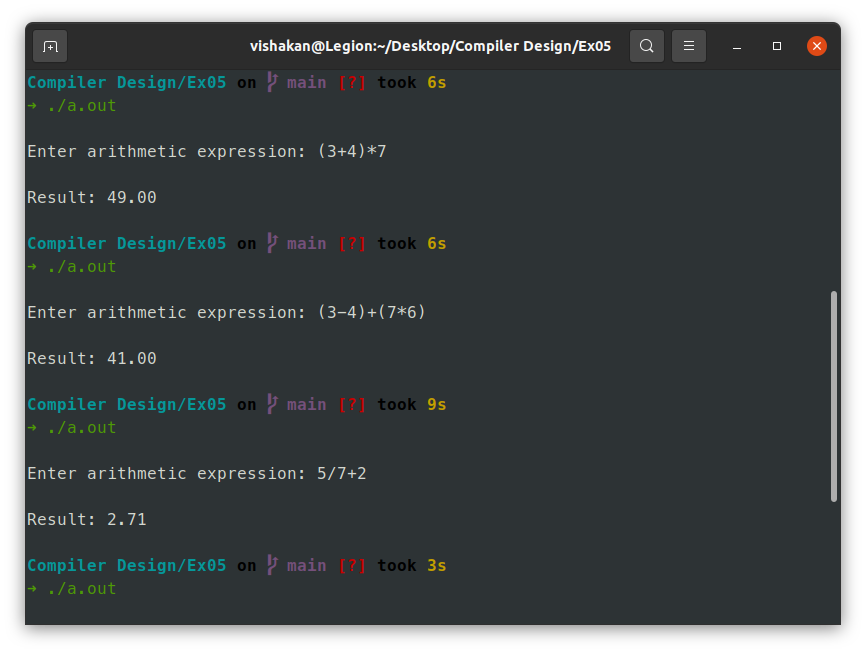
\includegraphics[scale= 0.5]{Output2.png}
\end{figure}

%Output
\newpage
\subsection*{\flushleft{Output 3:}}
\begin{figure}[h]
\centering
\caption{Console Output - 3.}
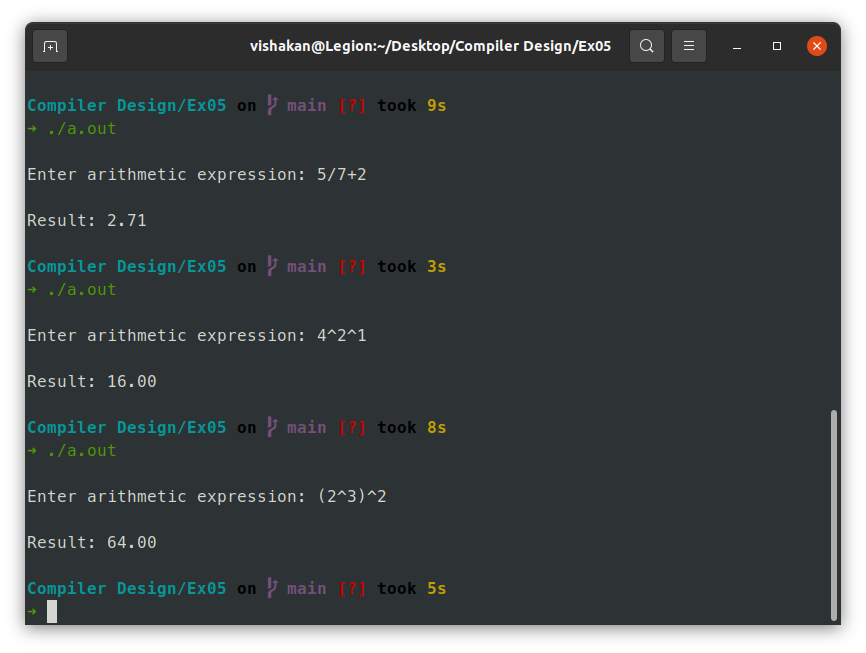
\includegraphics[scale= 0.5]{Output3.png}
\end{figure}

%Learning Outcome
\newpage
\subsection*{\flushleft{Learning Outcome:}}
\begin{itemize}

\item I learnt the basic theory behind \textbf{Yacc Parser Generator}.
\item I learnt that Yacc stands for Yet Another Compiler-Compiler.
\item I understood that Yacc is a LALR(1) parser.
\item I understood Yacc's basic syntax and programming logic.
\item I learnt that Yacc needs a Lex file along with it to work as intended, to detect and give the tokens to the Yacc parser.
\item I was able to visualize how the parser works with the scanner.
\item I learnt how to define a simple grammar in Yacc's syntax.
\item I was able to implement a parser with Yacc to mimic the features of a desk calculator with precedence logic.
\item I understood how to compile and run the Yacc and Lex file together.
\end{itemize}


\end{document}
